
In this exercise we will get to know the programming tool Node-RED which will be used 
for wiring together hardware devices, APIs and online services in new and interesting ways.

As the tool is primary picture based, there will not be much code in this exercise.
The exported \code{.json} of the Node-RED flow can be found in the sheet 2 folder of the 
\url{https://github.com/Smokey95/AIN_Ubiquitous_Computing} in the exercise section.


\section{Exercise 2.1; Hello World}

We will start with an basic example to get familiar with the tool b< just triggering a 
simple \code{Hello World} message.

\begin{figure}[h!]
  \centering
  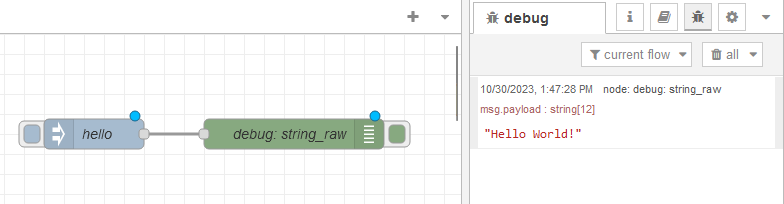
\includegraphics[width=1\textwidth]{exercise_node-red/exercise_1}
  \caption{Hello World}
  \label{fig:hello_world}
\end{figure}


\section{Exercise 2.2: Change Message}

In this exercise we will change the incoming \code{Hello World} message to \code{Hello Mars} and 
print it to the debug console.

\begin{figure}[h!]
  \centering
  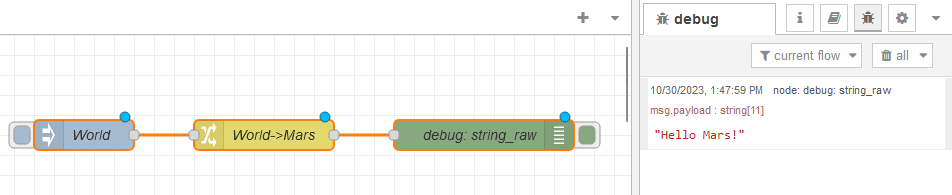
\includegraphics[width=1\textwidth]{exercise_node-red/exercise_2}
  \caption{Change Message}
  \label{fig:change_message}
\end{figure}


\section{Exercise 2.3: HTTP Request}

In this exercise we will use the \code{http request} node to get the current earthquake data from 
the \url{https://earthquake.usgs.gov/earthquakes/feed/v1.0/summary/significant_month.csv}.
It was decided to print the raw data to the debug console. Also the \code{change} node was used to 
change payload where the \code{mag} data was greater than 5.3 to \code{Panic!}.

\begin{figure}[h!]
  \centering
  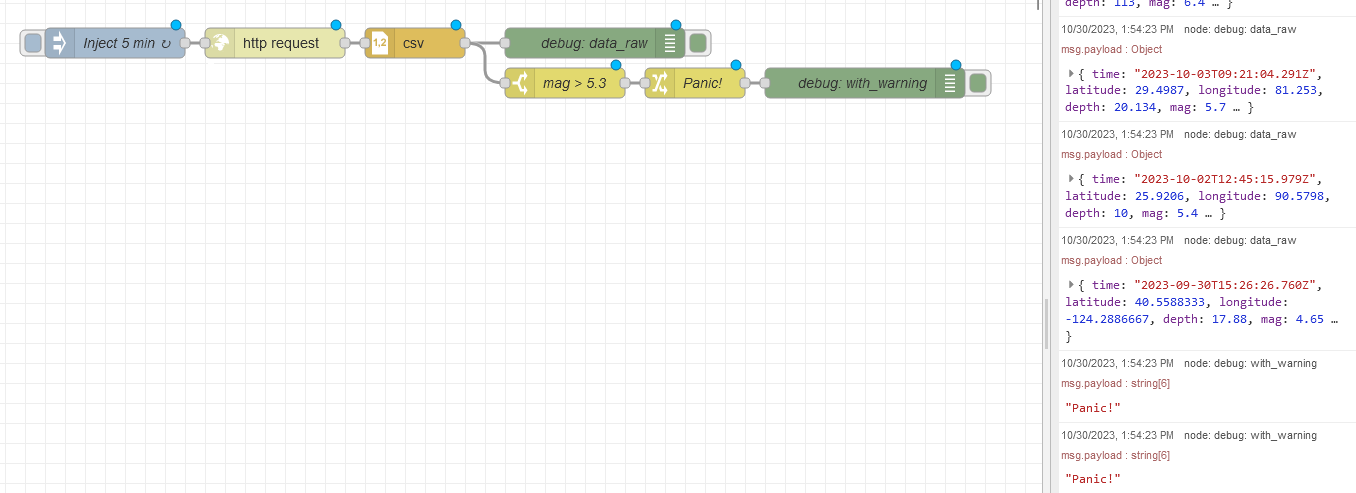
\includegraphics[width=1\textwidth]{exercise_node-red/exercise_3}
  \caption{HTTP Request}
  \label{fig:http_request}
\end{figure}


\section{Exercise 2.4: Dashboards}

In this exercise we will use the \code{dashboard} node to create a simple dashboard which will 
show the current time in several different formats.

\begin{figure}[H]
  \centering
  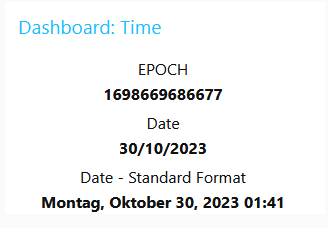
\includegraphics[width=0.8\textwidth]{exercise_node-red/exercise_4_dashboard}
  \caption{Dashboard}
  \label{fig:dashboard}
\end{figure}

\begin{figure}[H]
  \centering
  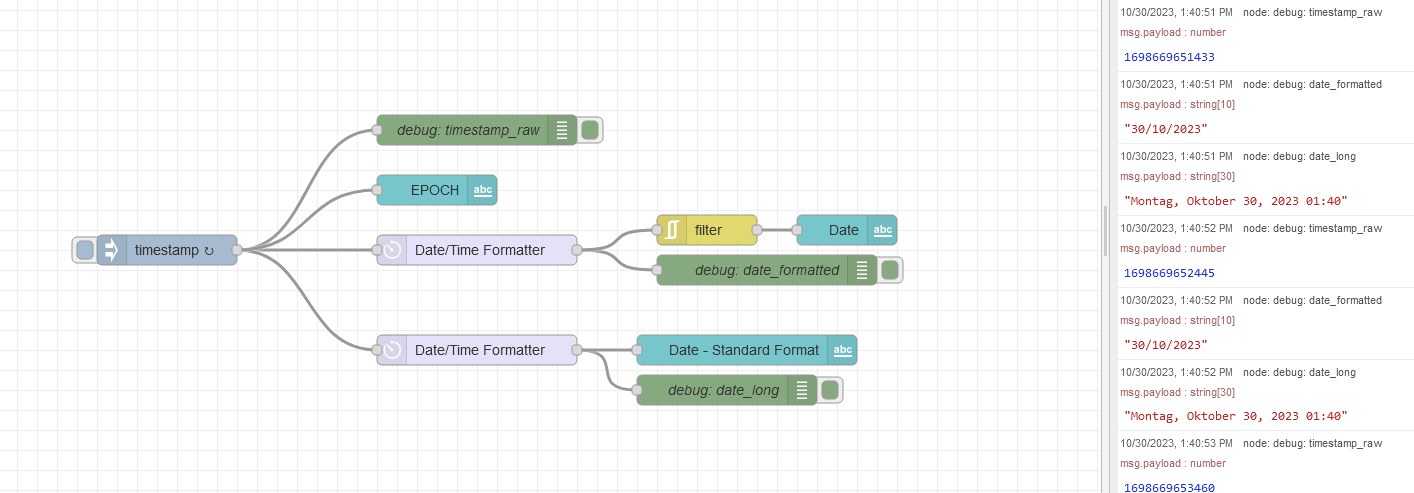
\includegraphics[width=1\textwidth]{exercise_node-red/exercise_4_node}
  \caption{Nodes}
  \label{fig:4_nodes}
\end{figure}

To display the date with written day name and month some time were spent to find the correct 
formatting of \code{dddd, MMMM DD, YYYY hh:mm} to display the timestamp like wanted.


\section{Exercise 2.5: LED Control}

In the fifth exercise we will use the \code{led} node to control the LED on the Arduino board as 
well as a hardware setup like seen [here](https://docs.arduino.cc/built-in-examples/digital/Button).

Notable is that instead of using the \code{5V} pin to power the LED, the \code{3.3V} pin was used 
cause even when operating the circuit with an pull down resistor the \code{5V} signal was bouncing.
Instead working with the \code{3.3V} signal was like expected.

The code below running on the Arduino board is as simple as expected.

\begin{minted}
  [
    frame=lines,
    framesep=2mm,
    baselinestretch=1.2,
    linenos
  ]
  {C}

  #include <WiFiNINA.h>

  const int button_pin = 4;
  
  void setup() {
    // Initalize LEDs
    pinMode(LEDR, OUTPUT);
  
    // initialize the pushbutton pin
    pinMode(button_pin, INPUT);
  
    Serial.begin(9600);
  }
  
  void loop() {
  
    static int debounce = 0;
    static String msg = "";
  
    // put main code here, to run repeatedly:
  
    if (Serial.available() > 0) {
      msg = Serial.readString();
    }
  
    if (digitalRead(button_pin) == HIGH || 
        msg.compareTo("1") == false){
      digitalWrite(LEDR, HIGH);       // Red LED on
      Serial.println(1);              // Writeback status for dashboard
    } else {
      digitalWrite(LEDR, LOW);        // Red LED off
      Serial.println(0);
    }
    
    delay(100);
  }
\end{minted}

The figure below shows the Node-RED flow with the hardware button on the breadboard pushed (notable 
cause software button is not pushed but LED is on) and the dashboard showing the correct status.

\begin{figure}[H]
  \centering
  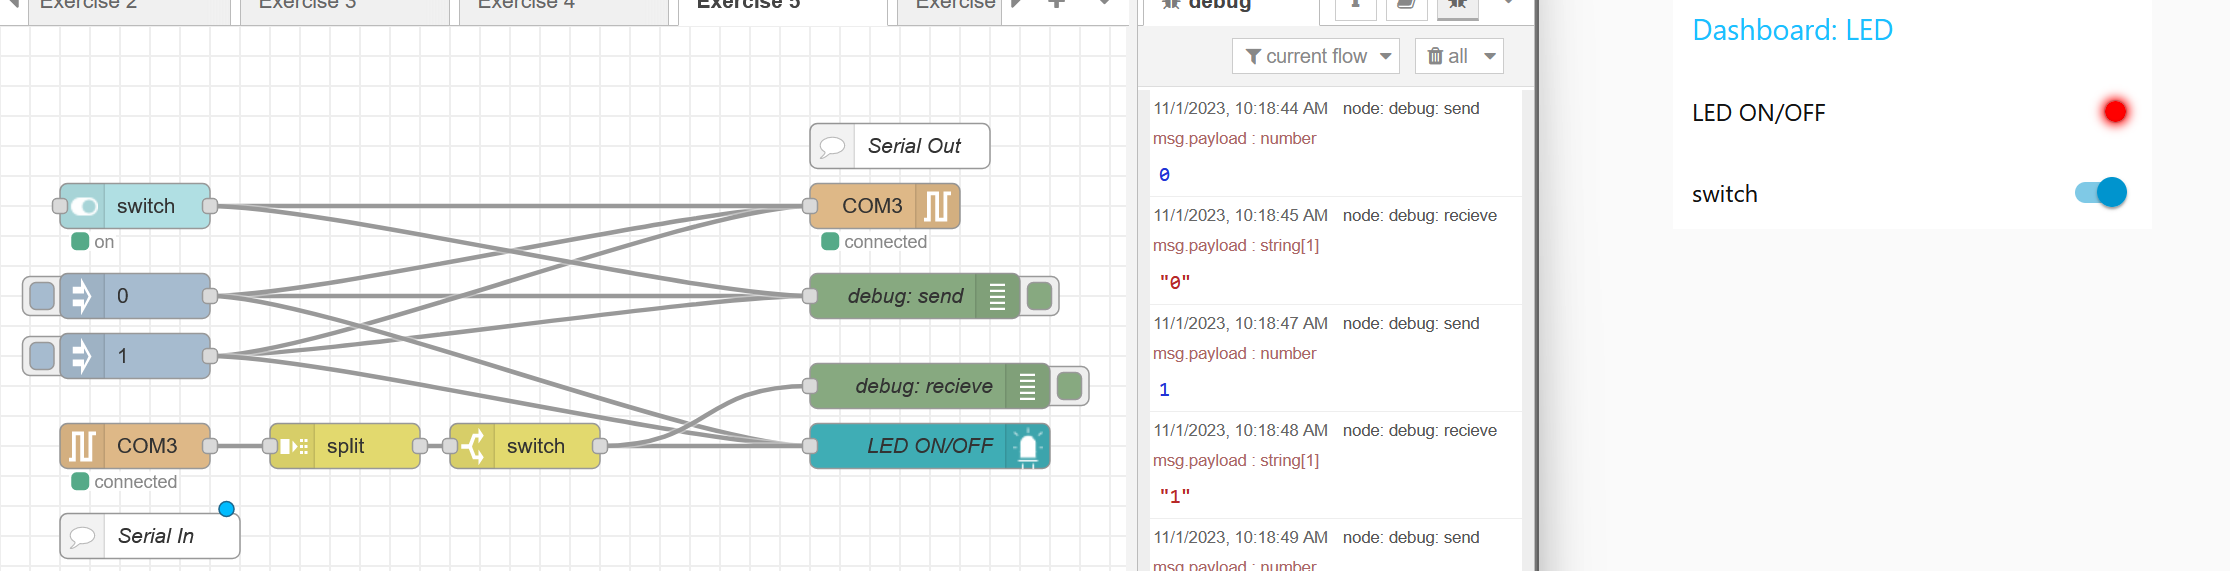
\includegraphics[width=1\textwidth]{exercise_node-red/exercise_5}
  \caption{LED Control}
  \label{fig:led_control}
\end{figure}


\section{Exercise 2.6: Temperature}

In this exercise we will use the \code{gauge} node to display the current temperature of the 
Arduino board. The temperature is measured using the internal temperature sensor of the Arduino. 
It was not a requirement but i tried to reuse the code from the first exercise with no changes 
leading to expanded node red flow.

\begin{figure}[H]
  \centering
  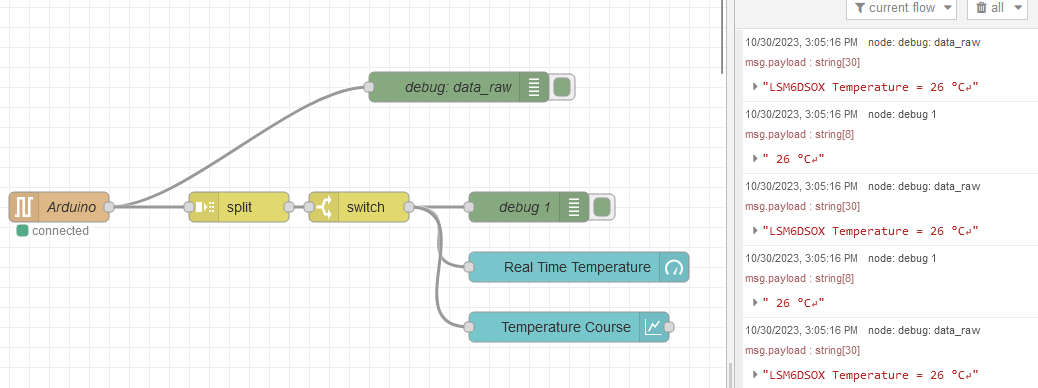
\includegraphics[width=1\textwidth]{exercise_node-red/exercise_6_full}
  \caption{Temperature}
  \label{fig:temperature}
\end{figure}

Like seen in the figure above, the Arduino board prints the current temperature to the serial port 
like in the code from the first exercise. To process this data the \code{split} node was used to 
split the incoming data stream and a \code{switch} node which will compare incoming data if it 
\code{contains °C} and only forward this data.

The resulting dashboard can be seen in the figure below.

\begin{figure}[H]
  \centering
  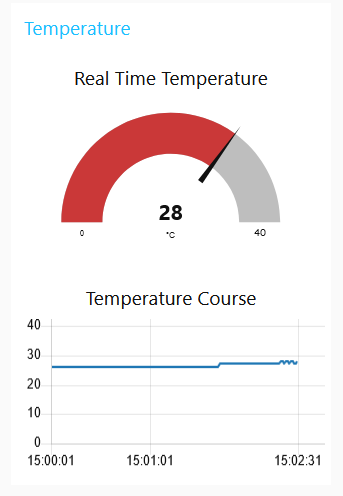
\includegraphics[width=0.5\textwidth]{exercise_node-red/exercise_6_dashboard}
  \caption{Temperature Dashboard}
  \label{fig:temperature_dashboard}
\end{figure}


\section{Exercise 2.7: MQTT}

In this exercise we will use the \code{mqtt} node to send the current temperature to a MQTT broker 
(hosted on \url{https://www.hivemq.com/try-out/}) and display it on a dashboard 
on \url{https://www.datacake.de/}.

Most effort was spent on this exercise cause it was not clearly described (or at least for me) 
how important the \code{topic} field is. This field has to match either in Node-RED config 
as well as on the datacake settings. Even after figure this out the data was not processed 
right so i created a second flow which send the data to the broker where it will be 
returned as \code{raw\_data}.

Also it has to be noted that this time the code of the Arduino was changed to send the 
temperature in a json styled format to the serial port. As most of the code was not changed 
only the relevant part is shown below.

\begin{minted}
  [
    frame=lines,
    framesep=2mm,
    baselinestretch=1.2,
    linenos
  ]
  {C}

  ...
  // Offset of ~30%
  float temperature_normalized = temperature_deg / 1.3;

  // Create a JSON-formatted string
  String jsonString = "{\"temp\": " + String(temperature_normalized) + "}";

  // Send JSON-formatted string over serial
  Serial.println(jsonString);
  ...

\end{minted}

This data will then rooted from the serial port to the \code{mqtt} node which will send it to 
the broker. Notice that the data will be send to two different topics. One topic is used to 
send data to an raw channel and the other one is used to send data to a formatted channel (see 
figure below).

\begin{figure}[H]
  \centering
  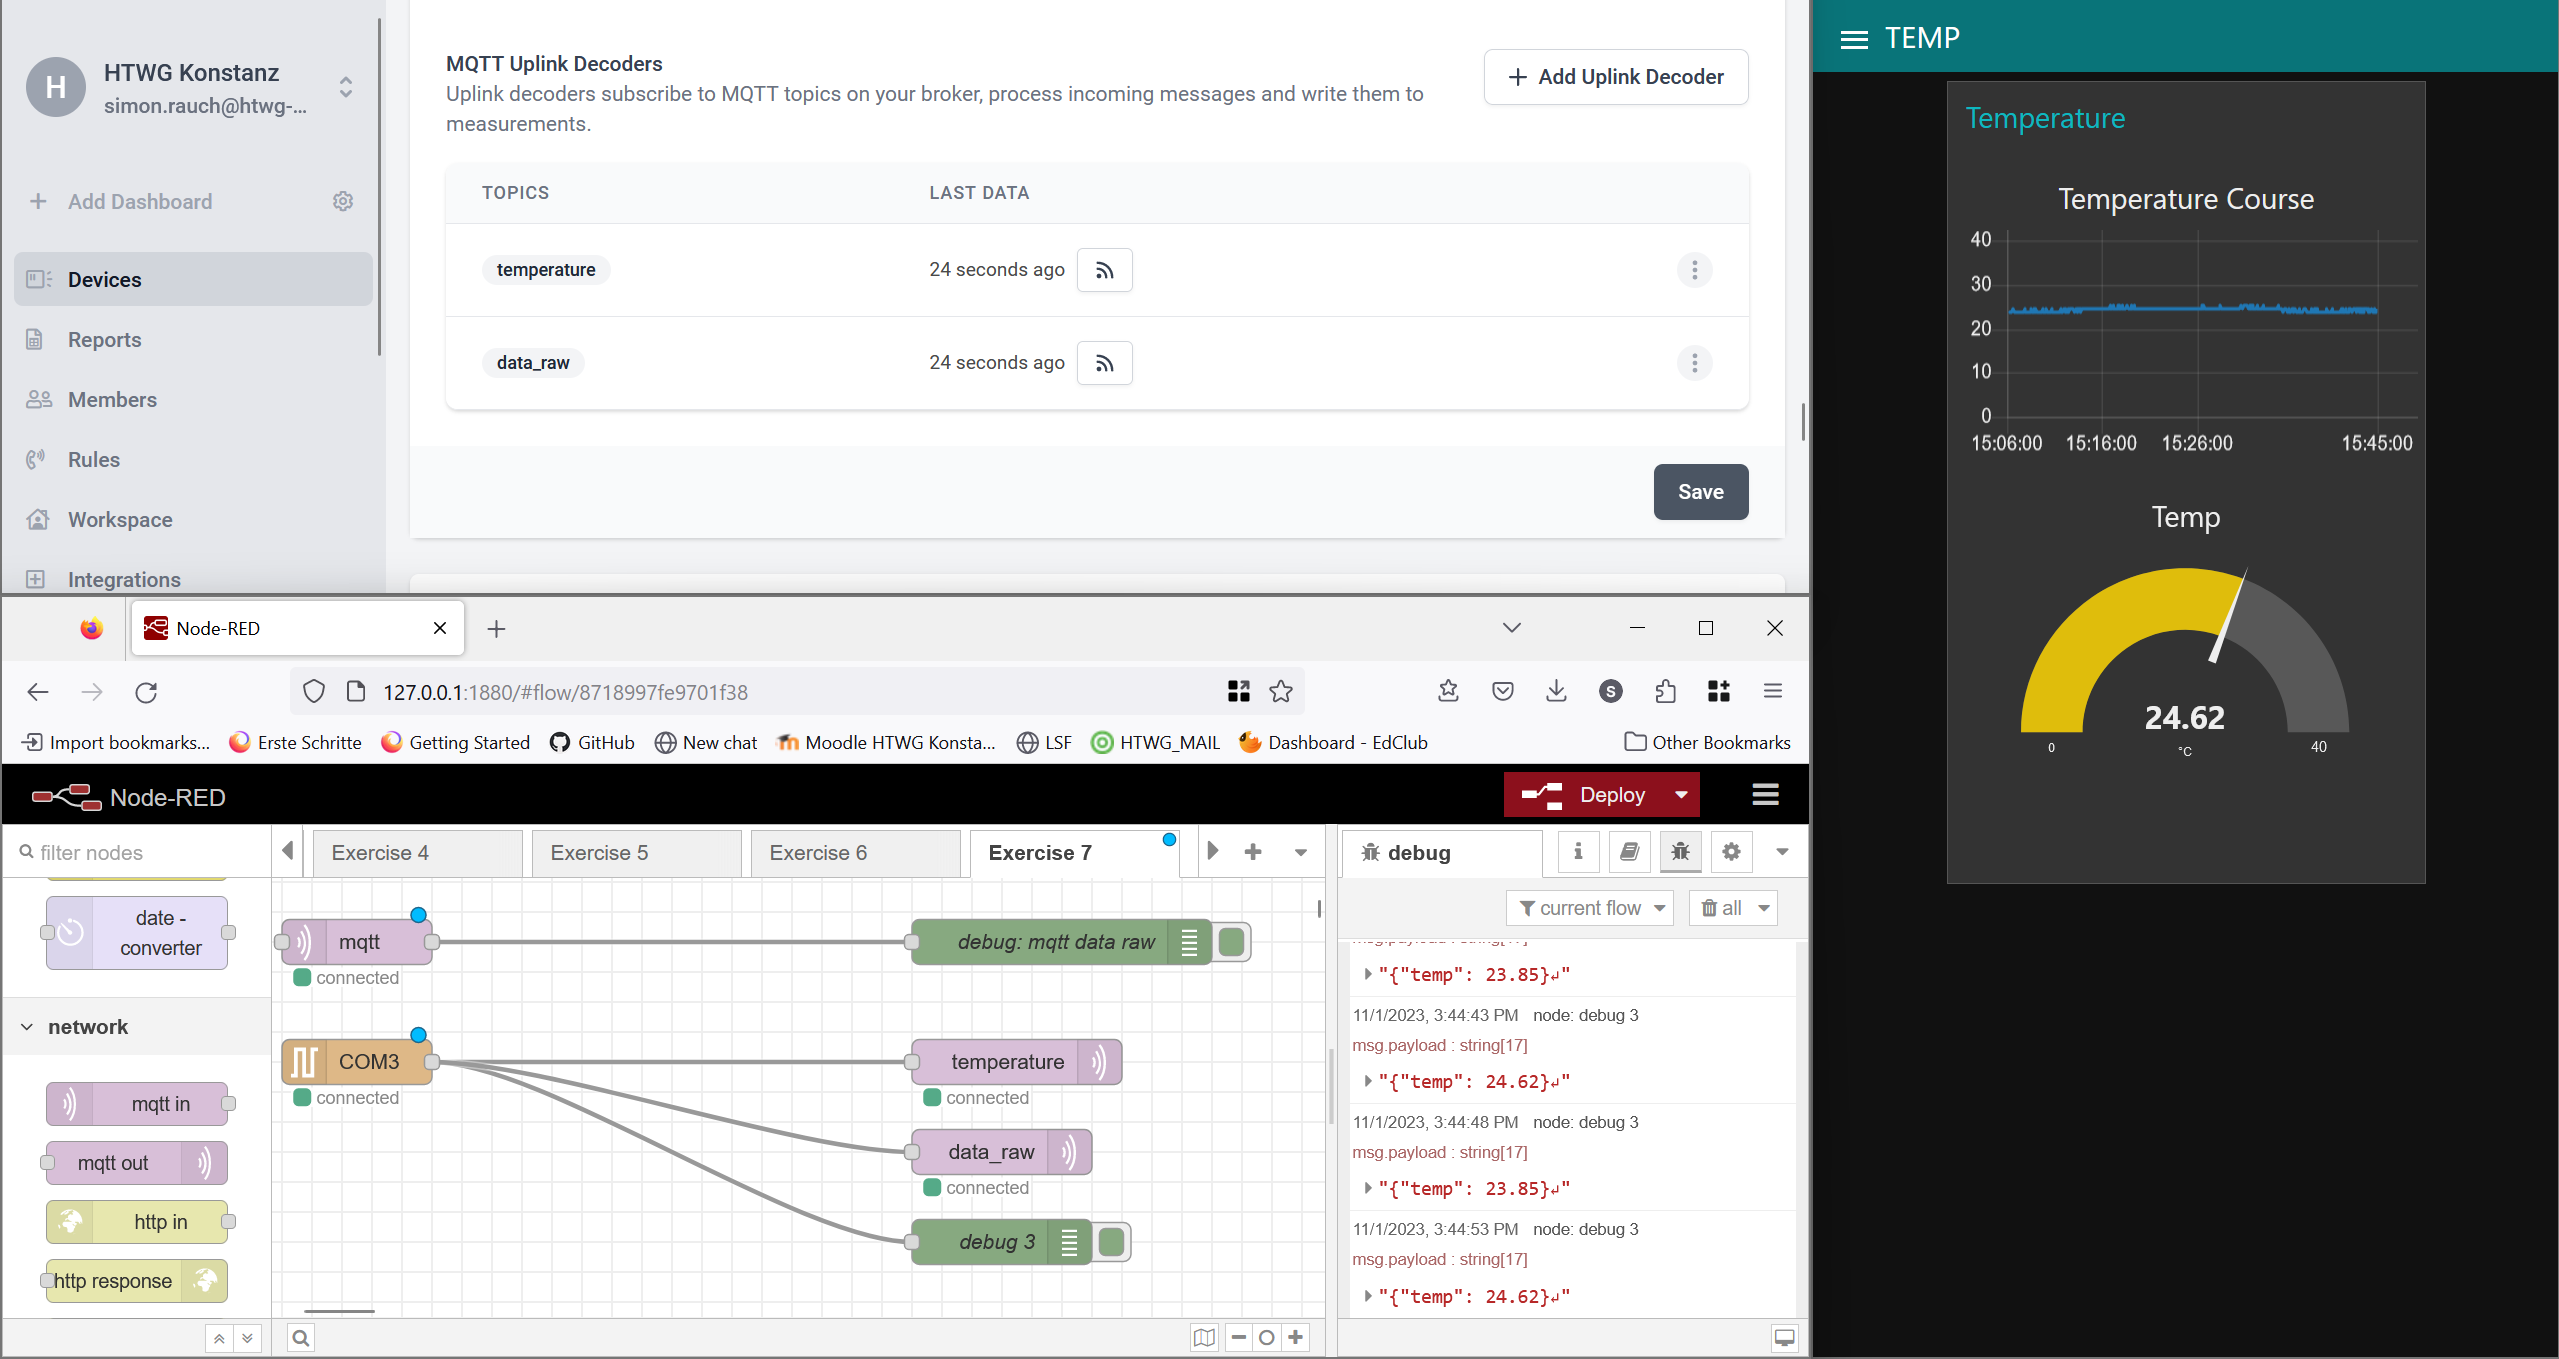
\includegraphics[width=1\textwidth]{exercise_node-red/exercise_7_data_raw}
  \caption{MQTT}
  \label{fig:mqtt}
\end{figure}

I spent some more time cause i does not why but even if the same data was send to both topics 
only the raw data was seen on datacake even if both Uplink decoder were the same. 
To waste no more time the decoder from the temperature channel was moved to the raw channel 
which worked fine and data was displayed on the dashboard.
Following you will see the java script to parse the data from the raw channel to the temperature field 
as well as the dashboard.

\begin{minted}
  [
    frame=lines,
    framesep=2mm,
    baselinestretch=1.2,
    linenos
  ]
  {javascript}

  function Decoder(topic, payload) {
    // Transform incoming payload to JSON
    payload = JSON.parse(payload);
    
    // Extract Temperature from payload, do calculation
    var temperature = payload.temp;
    
    // Forward Data to Datacake Device API using Serial, Field-Identifier
    return [
        {
            device: "e8aec33d-a641-4d25-a235-786fd1291a7b", // Serial Number or Device ID
            field: "TEMPERATURE",
            value: temperature
        },
    ];
  }
\end{minted}

\begin{figure}[H]
  \centering
  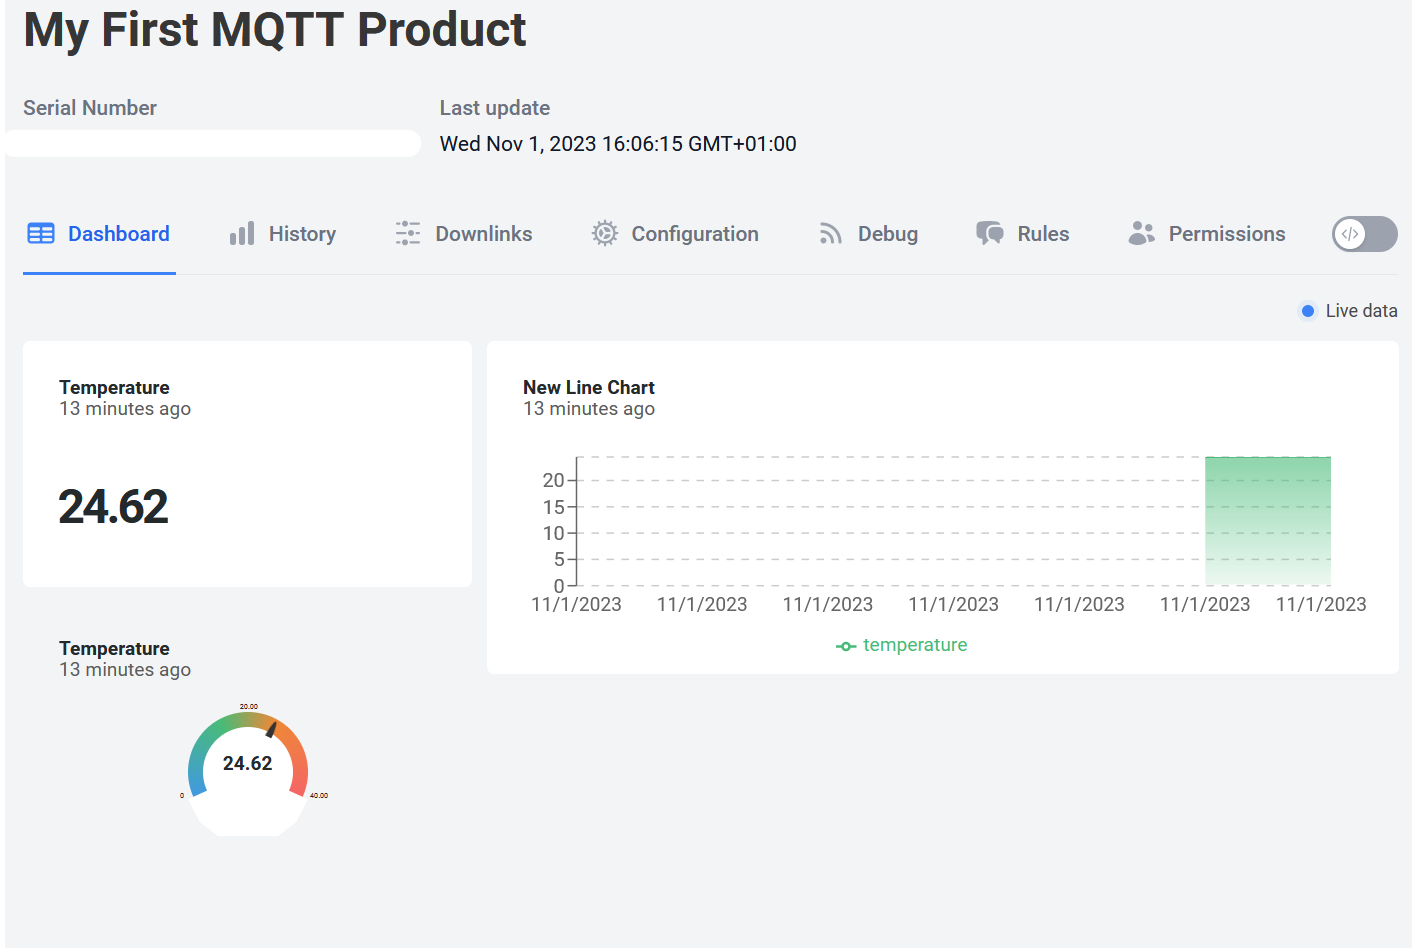
\includegraphics[width=0.8\textwidth]{exercise_node-red/exercise_7_dashboard}
  \caption{MQTT Dashboard}
  \label{fig:mqtt_dashboard}
\end{figure}

At the end of this exercise a downlink was setup to send a message to the Arduino board.
This was also a little bit frustrating but the config as well as the result can be seen below.

\begin{figure}[H]
  \centering
  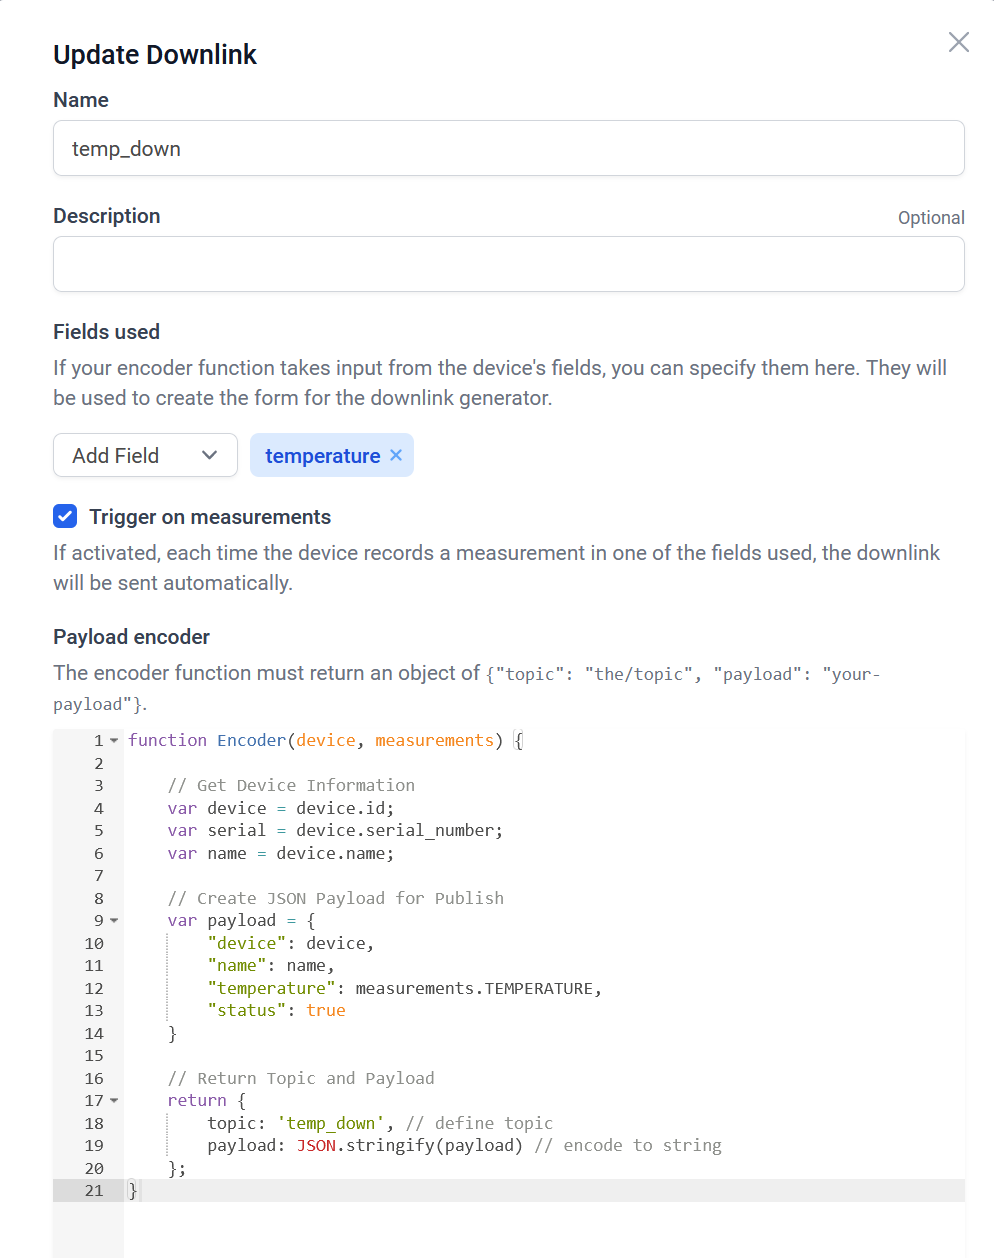
\includegraphics[width=0.7\textwidth]{exercise_node-red/exercise_7_downlink}
  \caption{MQTT Downlink}
  \label{fig:mqtt_downlink}
\end{figure}

\begin{figure}[H]
  \centering
  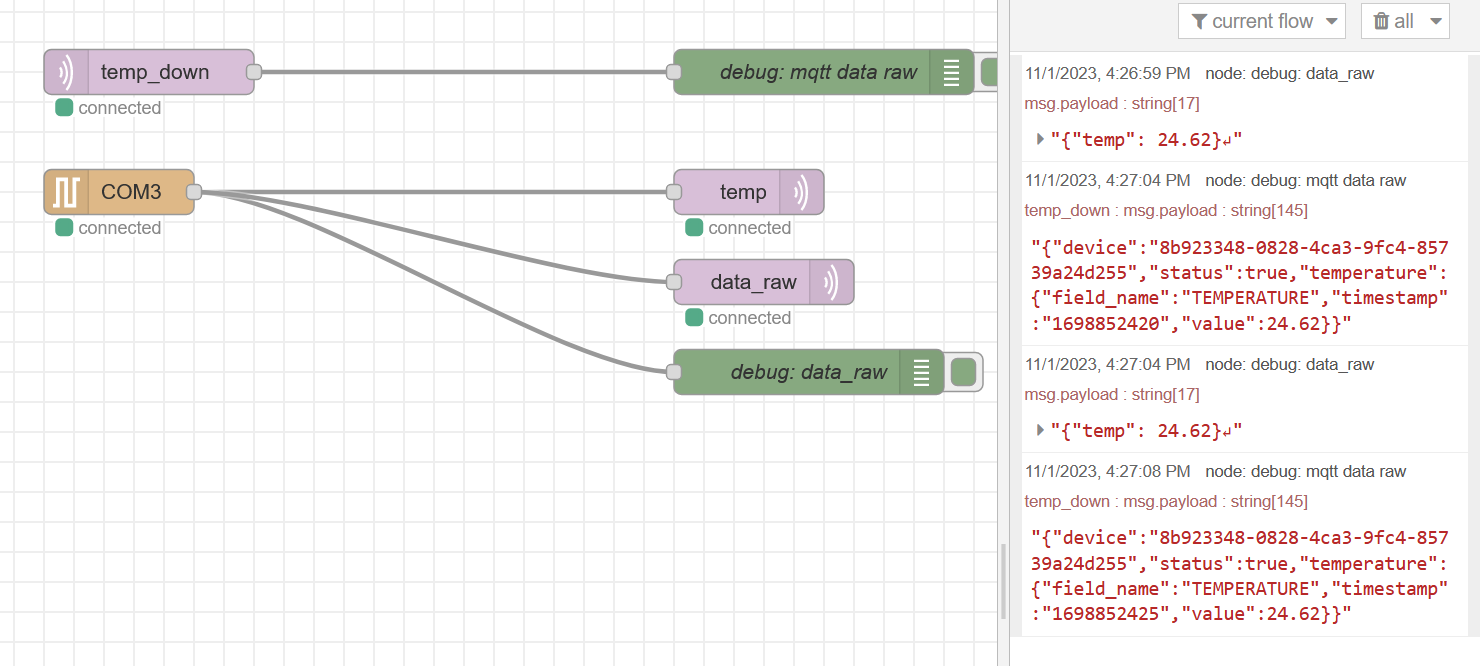
\includegraphics[width=0.8\textwidth]{exercise_node-red/exercise_7_data_down}
  \caption{MQTT Downlink Result}
  \label{fig:exercise_7_data_down}
\end{figure}


\section{Exercise 2.8: Cat door}

In the last exercise we will use the \code{mqtt} as well as the arduinos \code{gyroscope} to 
detect if the cat door is open or closed. The gyroscope is used to detect the angle of the door 
as well as the direction it is opened (detecting if cat is indoor or outdoor).
\newline
\newline
The code running on the arduino board is shown below.

\begin{minted}
  [
    frame=lines,
    framesep=2mm,
    baselinestretch=1.2,
    linenos
  ]
  {C}

  #include <WiFiNINA.h>
  #include <Arduino_LSM6DSOX.h>
  #include <MadgwickAHRS.h>

  Madgwick filter;

  void setup() {
    // Initialize serial communication and wait for port to open:
    Serial.begin(9600);
    while (!Serial) {
      ; // wait for serial port to connect. Needed for native USB port only
    }

    // Initialize the LSM6DSOX
    if (!IMU.begin()) {
      Serial.println("Failed to initialize IMU!");
      while (1);
    }

    filter.begin(104.00);

    // Initalize LEDs
    pinMode(LEDR, OUTPUT);
    pinMode(LEDG, OUTPUT);
    pinMode(LEDB, OUTPUT);

    digitalWrite(LEDR, LOW);    // Red
  }

  void loop() {
    float ax, ay, az;
    float gx, gy, gz;
    static int counter = 0;
    static bool state;
    static float temp = 0;

    // check if data is available every loop
    if(IMU.accelerationAvailable() && 
       IMU.gyroscopeAvailable()) {

      IMU.readAcceleration(ax, ay, az);
      IMU.readGyroscope(gx, gy, gz);

      // Update the filter with the latest data
      filter.updateIMU(gx, gy, gz, ax, ay, az);

      // Check the filter's roll for door movement
      if (filter.getRoll() > 5){
        state = true;
        digitalWrite(LEDR, HIGH); // Turn on LED if door is opened
      } else if (filter.getRoll() < -5) {
        state = false;
        digitalWrite(LEDR, HIGH); // Turn on LED if door is opened
      } else {
        digitalWrite(LEDR, LOW); // Turn off LED if door is closed
      }
    }

    if(!(counter % 100)){
      temp = get_temp();
      send_data(temp, state);
    }

    counter > 100 ? counter = 1 : counter++;
    delay(100);
  }

  float get_temp() {
    // Check if temperature is available
    if (IMU.temperatureAvailable())
    {
      int temperature_deg = 0;
      IMU.readTemperature(temperature_deg);

      // Offset of ~30%
      float temperature_normalized = temperature_deg / 1.3;

      return temperature_normalized;
    }
  }

  void send_data(float temp, bool in_out){
    // Construct JSON-style string
    String jsonString = "{\"temperature\": " + String(temp) + ", \"state\": \"" + (in_out ? "outdoor" : "indoor") + "\"}";
    Serial.println(jsonString);
  }

\end{minted}

Note that the sensor is checked in every iteration but the data is only send every 100th iteration to reduce 
the amount of data send to the broker. Also the data is send in a json styled format to the serial port.
\newline
\newline
Like seen in in the figure below the data is then send to the broker using \code{Node\-RED} where it is 
collected and displayed from \code{datacake}.

\begin{figure}[H]
  \centering
  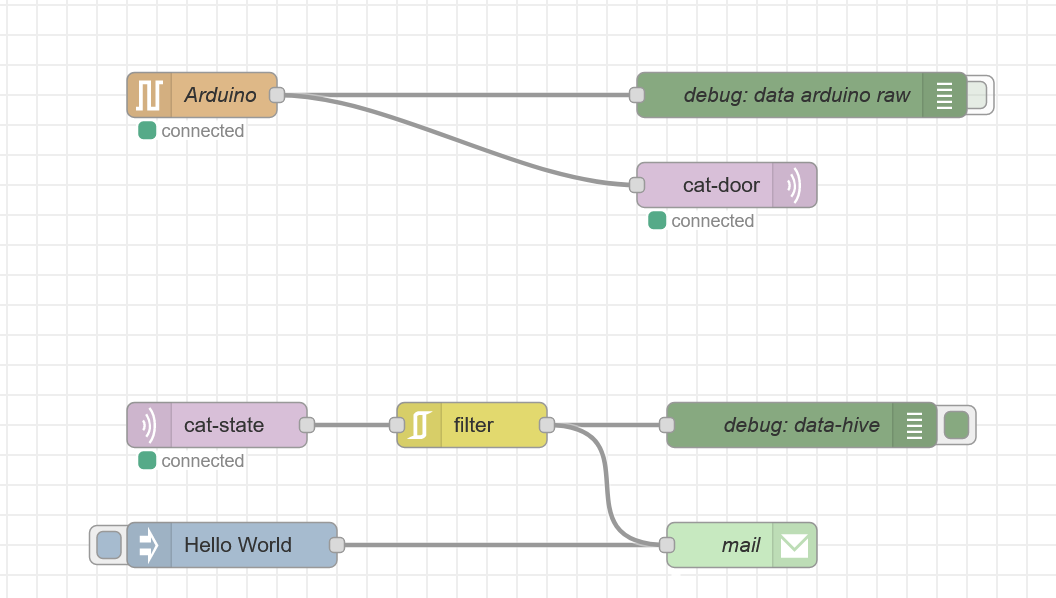
\includegraphics[width=1\textwidth]{exercise_node-red/exercise_8_node-red}
  \caption{Cat Door Note-RED Flow}
  \label{fig:cat_door}
\end{figure}

Also the data is send back from \code{datacake} to the \code{Note\-RED} flow using the \code{Downlink} feature 
which was introduced in the last exercise. This will trigger a \code{Mail} node which will send an email to 
the configured email address. (Cause of privacy reasons the \code{.json} file is not included in the repository 
cause it contains the email address.)

\begin{figure}[H]
  \centering
  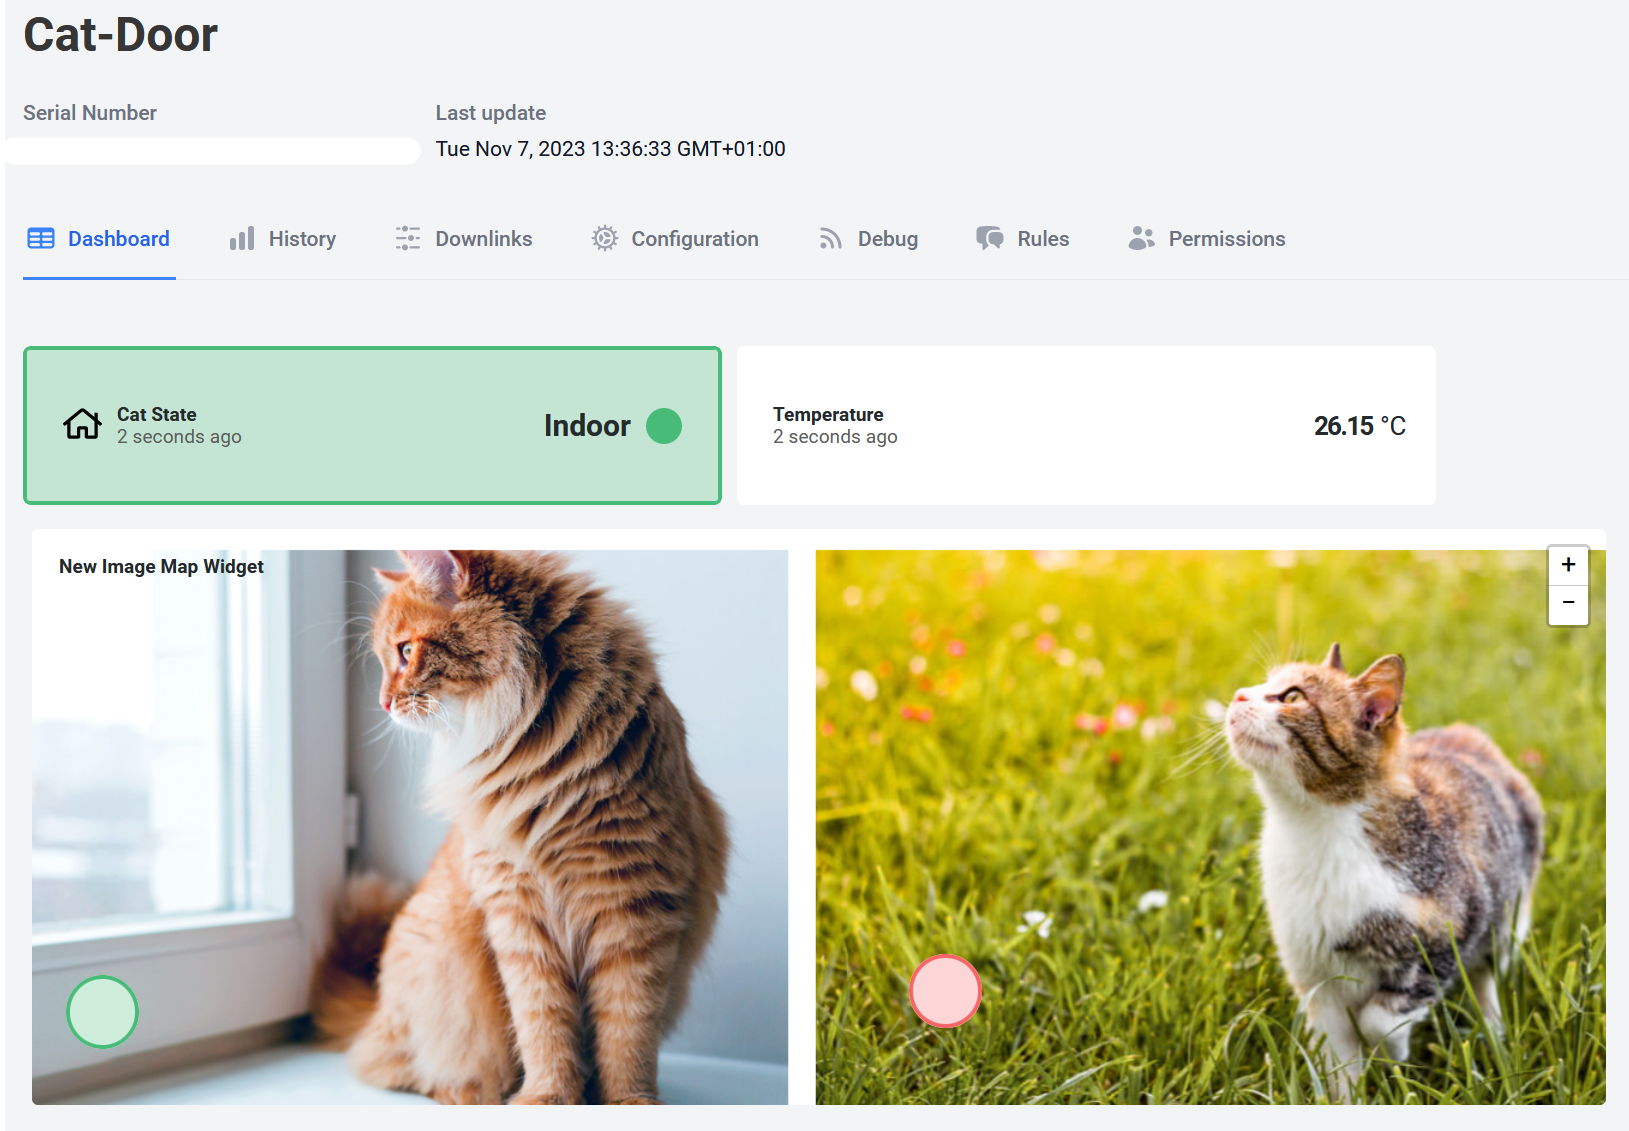
\includegraphics[width=1\textwidth]{exercise_node-red/exercise_8_dashboard}
  \caption{Cat Door Datacake}
  \label{fig:cat_door_datacake}
\end{figure}